\section{Effizienz der Regelmengen}

Um die Performance der einzelnen Regelmengen nachzuvollziehen, wurden die Regelmengen verglichen. Wie in Kapitel 4 beschrieben und unter 5.1 bemerkt, kann die Unvollständigkeit von RS-B2 (teilweise) durch den verwendeten Enumerator ExpandDAG verursacht worden sein. Daher wurde eigene Enumerator entwickelt und für die Test verwendet.

Wie im Folgenden zu sehen ist, ist der selbst implementierte Enumerator zwar sehr akkurat bei der Suche nach Planalternativen, jedoch wenig effizient. Um ein ähnliches Szenario wie in Kapitel 3 beschrieben durchführen zu können, wurde der Enumerator ExpandDAG nachimplementiert und ebenfalls in den Vergleich einbezogen.

\subsection{Vergleich des eigenen Enumerators mit ExpandDAG}


\begin{figure}[ht]
  \centering
  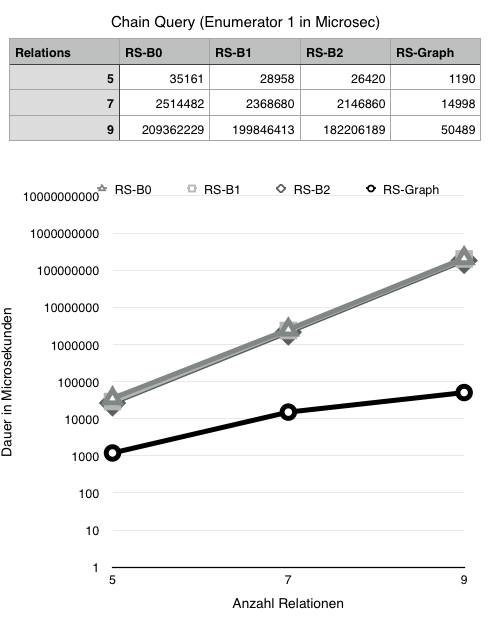
\includegraphics[width=0.5\textwidth]{05_ResultsEvaluation/00_media/ChainEnumerator1.png}
  \caption{Messergebnis des eigenen Enumerators bei kettenförmigen Anfragen}
  \label{chainQuery1}
\end{figure}

Bereits auf Abbildung \ref{chainQuery1} ist zu erkennen, wie ineffizient der Algorithmus ist. Im Vergleich der Regelmengen ist zu sehen, dass die Pellenkoft Regelmengen alle gemeinsam ähnliche Geschwindigkeiten erziehen. Jedoch ist RS-B2, der in diesem Fall vollständige Resultate generiert, der schnellste. Im Vergleich zu diesen Algorithmen ist RS-Graph erheblich schneller.


\begin{figure}[ht]
  \centering
  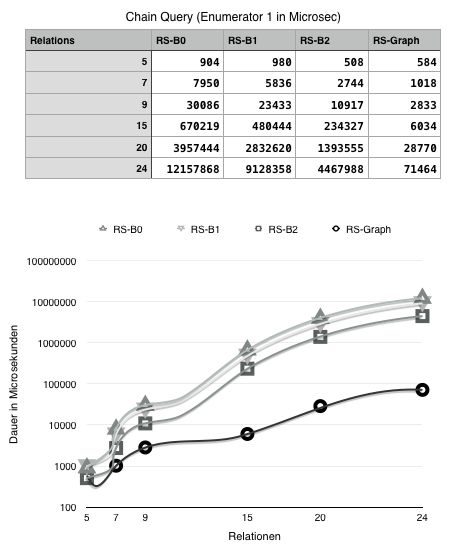
\includegraphics[width=0.5\textwidth]{05_ResultsEvaluation/00_media/ChainEnumerator2.png}
  \caption{Messergebnis des ExpandDAG bei kettenförmigen Anfragen}
  \label{chainQuery1}
\end{figure}


Mit Hilfe des zweiten Enumerators ExpandDAG wurden mehr Relationen zur Evaluation verwendet. Auch hier zeigt sich die Überlegenheit von RS-Graph.

Interessant ist insbesondere, dass im Vergleich zu den Kosten, die in Kapitel 3 zu sehen sind, RS-B2 nicht so kostenintensiv ist, wie die anderen Pellenkoft Regelmengen. Dieses Messergebnis verwundert, da in Kapitel 3 RS-B2 immer am schlechtesten abschnitt. RS-B2 schnitt dort mit exponentiellem Wachstum ab.

Das gute Abschneiden verwundert zwar im Kontext der Messungen aus Kapitel 3. Zieht man jedoch in betrachte, dass nach der Anwendung von Regeln maximal die Kommutativitätsregel ausgeführt werden kann, verringert sich die Anzahl der potenziellen Einsatzorte erheblich. Weniger Anwendungsmöglichkeiten können zu einer schnelleren Ausführung beitragen.





\subsection{Sternförmige, kreisförmige Abfragen}

Auch bei den Sternförmigen Anfragen wurde der eigene Enumerator verwendet. Wie zuvor gesehen, kann bei ExpandDAG möglicherweise nicht der vollständige Suchraum erforscht werden. Damit dieser Fehler nicht auftritt, wurde für die folgende Suche auch der eigene Enumerator eingesetzt.

Wie in Abb. \ref{starQuery123} zu sehen ist, sind die Ergebnisse ähnlich zu dem bisher gefundenen. Auch hier zeigt sich die bekannte Überlegenheit von RS-Graph. 


\begin{figure}[ht]
\centering
\begin{tabular}{|l|l|l|l|l|}
\hline
{\bf Relationen} & {\bf RS-B0} & {\bf RS-B1} & {\bf RS-B2} & {\bf RS-Graph} \\ \hline
5                & 79.381      & 75.210      & 70.986      & 913            \\ \hline
7                & 37.636.186  & 35.573.845  & 33.743.328  & 3.511          \\ \hline
\end{tabular}
  \caption{Messergebnis von sternförmigen Anfragen im eigenen Enumerator}
  \label{starQuery123}
\end{figure}


Auch bzgl. von kreisförmigen Anfragen (Abb. \ref{circle1} zeichnet sich ein ähnliches Bild. RS-Graph ist wie immer sehr performant. Die anderen Regelmengen hingegen nicht.



\begin{figure}[ht]
\centering
\begin{tabular}{|l|l|l|l|l|}
\hline
{\bf Relationen} & {\bf RS-B0} & {\bf RS-B1} & {\bf RS-B2} & {\bf RS-Graph} \\ \hline
5                & 82.395      & 79.395      & 43.331      & 1.566            \\ \hline
7                & 9.014.497  & 8.744.042  & 3.629.430  & 4.012          \\ \hline
\end{tabular}
  \caption{Messergebnis von zyklischen Anfragen im eigenen Enumerator}
  \label{circle1}
\end{figure}



\subsection{Fazit: Performance}

Wie zu erwarten war RS-Graph die effizienteste Regelmenge. Sie schnitt verglichen zu anderen Regelmengen immer besser als. Was jedoch stark verwunderlich ist, ist die Performance von RS-B2. Sie war besser als angenommen. Ebenfalls wurde festgestellt, dass die Suche nach einem Plan nicht nur abhängig von den Regelmengen, sondern auch von den Transformationsenumeratoren, die die Regeln auf die einzelnen Knoten anwenden.









